\documentclass{article}
\usepackage{graphicx}
\usepackage{geometry}
\usepackage[hidelinks]{hyperref}
% \usepackage{biblatex}

\geometry{
    a4paper,
    total={170mm,257mm},
    left=20mm,
    top=20mm,
}

% \bibliography{references}

\title{Single-actor bicycle crash classification guide}
\author{
  Benjam\'in Gonz\'alez\\
  \small{\href{mailto:b.gonzaleztoledo@tudelft.nl}{B.GonzalezToledo@tudelft.nl}}
  }
\date{\today}

\begin{document}

\maketitle

\begin{figure}[h]
    \centering
    \includegraphics[width=\linewidth]{class-mindmap-v2.png}
    \caption{Flowchart of bicycle crash classification.}
    \label{fig: flowchart}
\end{figure}

\begin{figure}[h]
    \centering
    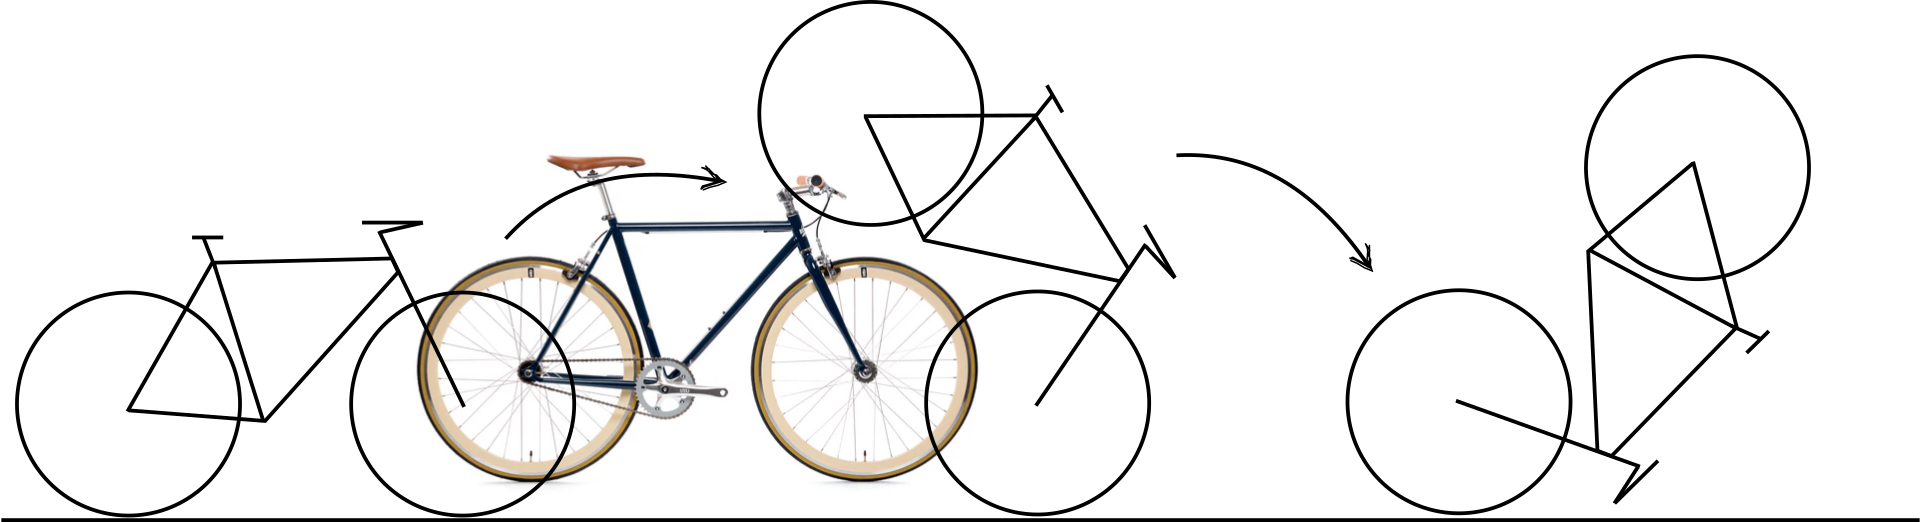
\includegraphics[width=\linewidth]{pitch-over.png}
    \caption{Simple diagram of pitch-over motion.}
    \label{fig: pitchover}
\end{figure}

\begin{figure}[h]
    \centering
    \includegraphics[width=\linewidth]{roll-over.png}
    \caption{Simple diagram of roll-over motion.}
    \label{fig: rollover}
\end{figure}
\section{Introduction}

This document aims to guide you to understand the proposed classification \cite{Jac04} of single-actor bicycle-crashes and label the samples sent to you.

\subsection{What is a Single-actor bicycle crash?}

A single-actor bicycle-crash is an event where the normal riding of the bicycle is disrupted and ends in a crash with no other road users involved.

\section{Bicycle dynamics-oriented classification}

The proposed workflow to classify the crash according to the observed characteristics is composed by three sub-categories: motion, interaction and mechanism (see Figure \ref{fig: flowchart}).

\subsection{Motion of the bicycle}

This is related to the main motion of the rear frame of the bicycle while the crash is occuring.
%
Due to the dynamics of the bicycle, and following the common simplification to its analysis, we find two main motions related to the degrees of freedom: pitch-over and roll-over.
%
Additionally, the roll-over motion includes its own sub-classification according to the direction of rotation with respect to the initial motion.
% 
Please visit \url{https://youtube.com/shorts/_etyqSpH10c?feature=shared} to watch an example of a crash where the final rotation is in the opposite direction of the initial motion.
%
This is particularly challenging to represent in a normal drawing so the visual explanation is on the make.

\begin{itemize}
    \item \textbf{Pitch-over (P):} The main characteristic of this motion is one of the wheels lifting from the ground and following a trajectory that finishes with the front wheel behind the rear wheel.
    \item \textbf{High-side (H):} Characterised for a sudden deceleration of the wheel while in lateral motion, which leads to a violent roll motion in the opposite direction of the initial motion.
    \item \textbf{Low-side (L):} The human-bicycle system follows an excessive roll motion in the same direction as at the beginning.
\end{itemize}

\section{Force}

This category refers to the forces excerted on the human-bicycle system, where we find external perturbation or no external perturbation.

\begin{itemize}
    \item \textbf{External forces (E):} Lorem ipsum.
    \item \textbf{Rider forces (I):} Lorem ipsum.
\end{itemize}

\section{Mechanism of crash}

\subsection{External mechanisms}
\begin{itemize}
    \item \textbf{Tyre forces:}
    \item \textbf{Aerodynamic forces:}
    \item \textbf{Body excerted forces:}
\end{itemize}

\subsection{Rider mechanisms}
\begin{itemize}
    \item \textbf{Brake input:}
    \item \textbf{Steering torque:}
    \item \textbf{Power input:}
\end{itemize}

\subsection{Location}

Lorem ipsum ...

\section{Force characteristics}

Lorem ipsum ...

\section{Example}

Let's do an example using the following video \url{https://youtube.com/shorts/VZibdrdhdgM?feature=shared}.

First, it is observed that the main motion of the bicycle in the crash is related to roll angle.
%
Additionally, it is in the same direction of the beginning of the motion.
%
Therefore, this corresponds to the category low-side (L).


Second, there are no visible perturbations that fit into the classification.
%
For this reason, we classify it as non-externally perturbed (0).


Third, the mechanisms that best fits into the scenario is slide (S).
%
After a detailed examination, it is reasonable to assume that the event started from the front wheel slide (F).


Finally, the classification of this crash would be \textbf{L0-SF}, front slide low side.

\begin{thebibliography}{9}

    \bibitem{Jac04} Elin K. Jacob (2004):  Classification and Categorization: A Difference that makes a Difference. Graduate School of Library and Information Science. University of Illinois at Urbana-Champaign. \url{http://hdl.handle.net/2142/1686}

\end{thebibliography}


\end{document}
